\chapter{Background}

Thanks to a protective atmosphere, Earth can withstand impacts from dust-sized to boulder-sized objects traveling faster than bullets without so much as a dent on Earth's surface.
While most of these near-Earth objects are extremely small and don't leave much of a trace, the larger objects can leave a light trail visible from Earth's surface as they burn up in our atmosphere.
In this chapter, we will discuss the classification of near-Earth objects, the camera system and equations we will use for our analysis, the existing photometry tools we have, along with other existing surveys.


\section{Description of Fireballs}

When considering types of near-Earth objects, many names come to mind.  
Asteroids, meteors, meteorites, and fireballs are often used interchangeably. 
However, there are several key distinctions between these objects.  
Asteroids are the largest of this group and are generally over $10$m in diameter \cite{steel_meteoroid_1996}. 
These large objects are responsible for large craters that are visibly present on the moon.  
Meteoroids are anywhere between $10 \mu$m and $10$m and are drastically more common than asteroids.  

Meteoroids that pass through earth's atmosphere become meteors.
As meteors pass through the atmosphere, they begin to ablate, or release light.  
This phenomena happens because the interactions between the meteor molecules with the air molecules produce lots of energy, some of which goes into the production of light.
This light can be measured in terms of apparent magnitude.
Magnitude is represented on a $\log_10$ scale and dimmer objects are represented by high numbers while brighter objects are lower.  
If the meteor releases visible light below an apparent magnitude of $-4$ qualify as bolides, or fireballs.
For reference, Venus is a magnitude $-4.4$ planet while the dimmer Jupiter has a magnitude of $-2.1$ \cite{rao_venus_nodate}.


If an object is massive enough to withstand the pressures of Earth's atmosphere and make it to the surface of Earth, it is classified as a meteorite. 
These are extremely uncommon, but provide valuable information about the rock's origin.
Figure \ref{jed} shows the relationship between these 4 objects.

\begin{figure}[ht!]
  \centering
  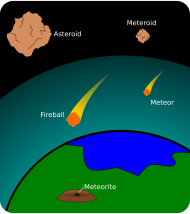
\includegraphics[scale=0.5]{images/jedmasterpiece.png}
  \caption{A depiction of near-Earth object classification.}
  \label{jed}
\end{figure}

We may further classify near-Earth objects into two categories: sporadic events and meteor shower events. 
Meteor showers occur when Earth's orbit crosses paths with the orbit of a collection of debris. 
Such collections often orbit large masses such as Jupiter or the sun \cite{trigo-rodriguez_2006_2007}.  
For example, the Perseid meteor shower has a highly elliptical orbit around the sun as seen in Fig. \ref{perceid}.  
A majority of the composition of these showers stems from the decomposition of comets throughout space.  

\begin{figure}[ht!]
  \centering
  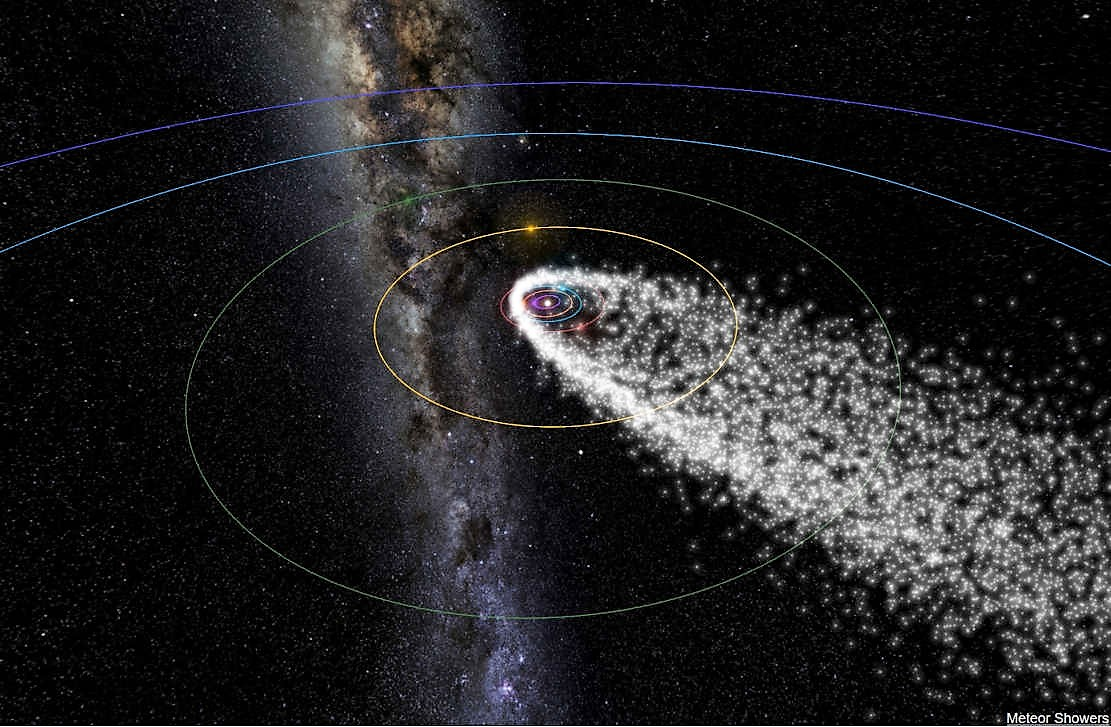
\includegraphics[scale=0.7]{images/persiod_shower.jpg}
  \caption{The Perseid meteor shower and its relation to our solar system.}
  \label{perceid}
\end{figure}

In contrast, there is debris in space that is not connected to any meteor shower. 
These are called sporadic events. 
Because gravity tends to bring objects together, we see mostly collections of debris.
However, when objects escape their collection due to other interactions (gravitational or electromagnetic), they still have a chance of colliding with Earth.

Studying these near-Earth objects can give us good estimates for how many objects you might expect to see pass through a given area of space within a specific amount of time. 
This measurement is called flux.
By determining flux, we can more accurately predict the likelihood of objects in space being hit by near-Earth objects. 
Although the case may have been an extreme one, the space satellite Olympus was struck and destroyed by a meteoroid during the Perseid meteor shower in 1993 \cite{bobrowsky_comet/asteroid_nodate}.
Additionally, given the relationships between the number of objects hitting earth per time for different objects, we can estimate the probability of extremely large impacts on earth.
These estimates, similarly to predictions surrounding volcanic or earthquake activity, give us insight into past events and help us foresee likelihoods of future events.








\section{The D6 AllSky Camera}

The Willamette University D6 Allsky camera was created in 2016 to capture the paths of fireballs throughout the night sky. 
The aim of the project was to create an economically feasible and easily mobile observational system.
By using a state-of-the-art camera system, a structure, some necessary reinforcement materials, and a programmable microcomputer, Kyle McSwain alongside Dr. Jed Rembold were able to get a functioning camera system \cite{mcswain_using_2016}. 
The camera resembles a Star Wars droid, and acquired its name from this inspiration.
This resemblence (paired with a little imagination) is shown in Fig. \ref{droid}.
The D6 Allsky camera is currently functioning properly and has been taking data since the summer of 2018.  
Below, we will discuss the composition of the D6 AllSky Camera while also highlighting what makes it significant.

\begin{figure}[ht!]
  \centering
  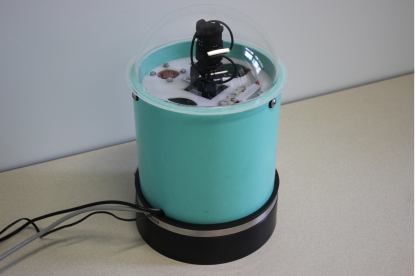
\includegraphics[scale=0.7]{images/allsky_camera.png}
  \caption{The Willamette D6 AllSky Camera (2016) \cite{mcswain_using_2016}.}
  \label{droid}
\end{figure}

\subsection{Composition}

The operational aspect of the D6 AllSky Camera is composed primarily of 5 different pieces: the camera housing, CCD camera, thermostat, digitizer, and the microcomputer (used to be raspberry pi).
The acrylic dome and PVC shell are both vital parts of our system. 
The dome itself is a transparent half sphere that sits on top of a PVC cylinder that holds the system together.
It acts as a protective layer between the camera and the outside environment.  
Without this feature, the camera would be subject to dew, bug contamination, and other undesired interferences.

The CCD camera is perhaps the most important feature of the camera.  
The Watec $902$H$2$ CCD camera uses a fish-eye lens to capture incident light from the night's sky.  
It was chosen due to its extremely high sensitivity and resolution \cite{mcswain_using_2016}.
While some fireball camera stations are composed of multiple high resolution, more narrow lensed cameras, the D6 AllSky system only contains one camera mostly for economic reasons.  
This camera was chosen in part due to its compact size, an important part of the highly valued versatility of our system. 
The camera is kept at a relatively constant temperature by a thermostat and a fan system. 
Because of its constant use throughout the night, the system itself can get very warm and therefore needs some thermal regulation.

The digitizer is the tool that allows us to transfer camera information to the microcomputer efficiently.  
The camera outputs analog signals which through the digitizer are converted to digital signals.
Through cable connections, the digitizer then sends the new output to the microcomputer where the initial analysis is run. 
The microcomputer takes the frames from the camera's running video and scans for systematic changes in brightness.
These changes then trigger the recording and storage of a new video, which is saved for further photometric analysis.
By combining these parts into one system, we are able to capture and catalog fireball events.

\subsection{Uniqueness}

While there are several similarities in the composition of our AllSky camera to existing systems, there are several key differences.
The most prominent of these are the size, versatility, and cost of our system.
Around the size of a basketball, the D6 AllSky camera is extremely compact.  
Not only is it small, but it only relies on a single power chord for power.  
Because of this, the camera can be relocated to any setting that has a power source.  
We should note that an external portable power source is a potential upgrade to this system that may take place in future creations.
Most other systems are rooted to extremely powerful computers that have little to no mobility as shown in Fig. \ref{immobile}.

\begin{figure}[ht!]
  \centering
  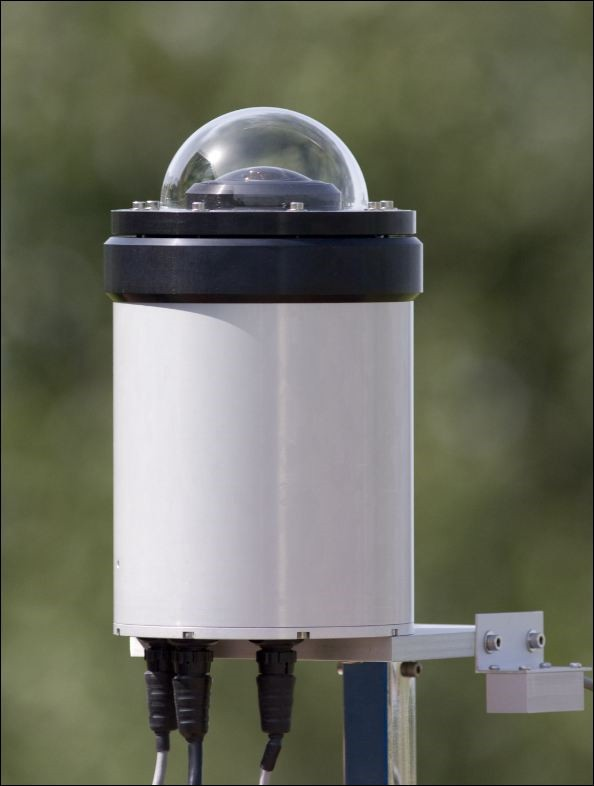
\includegraphics[scale=0.3]{images/othercam.jpg}
  \caption{An entrenched alternative AllSky camera.}
  \label{immobile}
\end{figure}

This presents issues related to being rooted in one location.
For example, if a tree were to grow near the camera, it would need to be chopped down or the entire system may need to be relocated.
With the lightweight and easily movable D6 AllSky camera, relocation is not a difficult process.

Most importantly, the D6 AllSky camera is a less expensive alternative to other fireball analysis tools.  
The ingenuity of running initial analysis on a microcomputer allows the D6 AllSky camera to cost a fraction of what professional systems cost.
Although large professional organizations produce copious amounts of wonderful data, in the field of fireball research, non-intensified systems outnumber intensified systems $2:1$ \cite{gural_review_2005}.  
Providing this cost efficient alternative could be a great way to expand the field of fireball research and in turn provide a better understanding of the near-Earth objects in our solar system.






\section{Photometry}
After collecting videos of potential fireballs, next comes the task of analyzing the videos.
Luke Russell, advised by Dr. Jed Remobld created a photometry program that allows us to get a calibrated intensity light curve for a given video of a fireball.
Simply running a fireball video through his interactive GUI allows us to access information about luminous properties of the fireball.
However, limitations to our photometry must be taken into account.
False positives, extinction, and other bothering problems must be accounted for while creating our fireball catalog.

\subsection{Existing photometry tools}
When running a video through the existing photometry script, the user must interact with the program.
After selecting a file to run through the program, the user must find the frame in the video which the fireball first becomes visible.  
Then, the user must left click on the fireball.
After this, the user must right click on a reference star with a known magnitude.
This step requires a bit of knowledge and will hopefully be automated throughout this project.
After selecting both of these and entering in the known magnitude of the reference star, the program will automatically track the fireball throughout the following frames.
By using Gaussian fits to the photometric data, the program is able to center its view on the fireball and determine its size throughout its path.
Throughout this process, the video also sums the photon counts for each fireball pixel for each frame.
This photon count gives us the magnitude of the fireball at a given point in it's path.
Doing this for each frame results in a light curve that shows the magnitude as a function of time.  
By using relations given in the Analysis section, we are able to calibrate the magnitude and from that calculate the intensity which yield the valuable light curve.
From this light curve, we can then move on to further analysis.

\subsection{Planes, \st{Trains} Bugs, and \st{Automobiles} Extinction}

\begin{figure}[ht!]
  \centering
  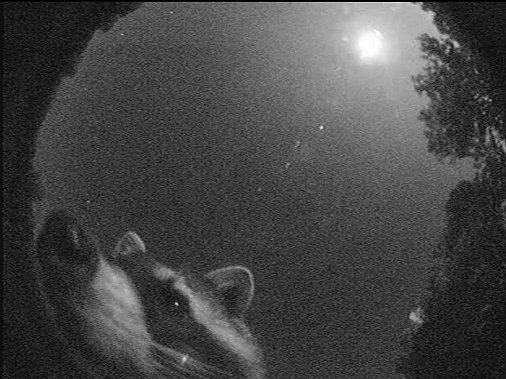
\includegraphics[scale=0.3]{images/racoon_cam.jpg}
  \caption{A fireball/raccoon hybrid.}
  \label{raccoon}
\end{figure}

While it is able to capture fireballs, the D6 AllSky camera still picks up a great deal of false positives.
In an initial sample of over $700$ videos, only $2$ of them contained real events.
The vast majority of the videos were of bugs crawling across the acrylic dome.
Because the bugs are illuminated by nearby light, they appear to be bolides traveling across the screen.
Many bugs are featured in several videos as they have a tendency to move, stop somewhere, and move again.
While this is somewhat problematic, we aim to implement several steps to limit the number of false positive bug cases.

In addition to bugs, airplanes, satellites, and iridium flares provide false-positive videos.
Their near-linear motion and bright presence are an instant trigger for the fireball detection.
This is a more difficult bug to fix when compared to the bug bug :).
These two cases are just small examples of false positives that result in difficult data to process.

\begin{figure}[ht!]
  \centering
  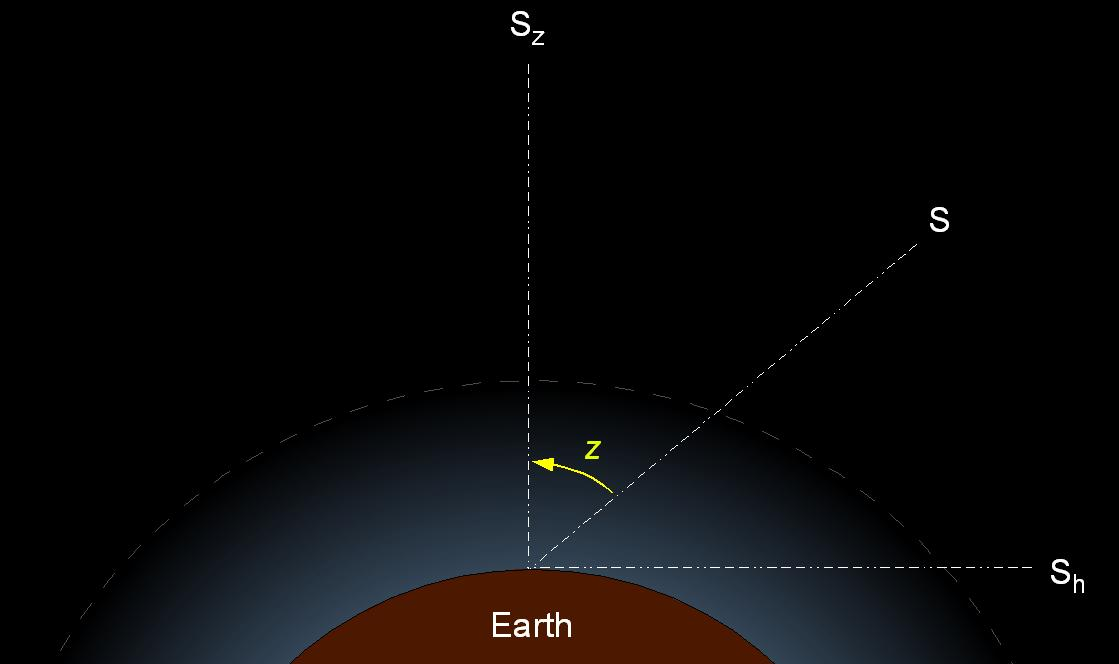
\includegraphics[scale=0.4]{images/extinction.JPG}
  \caption{A depiction of atmospheric extinction.}
  \label{extinc}
\end{figure}

A larger problem in data analysis stems from the phenomena of atmospheric extinction.
As shown in Fig. \ref{extinc}, we observe that when looking close to the horizon (S$_h$ in the image), light must travel through a larger volume of atmosphere than it does for an observation close to the zenith (S$_z$ in the image).  
Because the light travels through more atmosphere, more of the light is absorbed by gases or scattered by air particulates \cite{noauthor_atmospheric_nodate}.
A prime example of atmospheric extinction is that of the sun. 
When directly overhead, the sun is at its brightest and one should never directly look into it.
However, close to the horizon, the sun appears more red and can be looked at directly.
Because a rising or setting sun's rays must travel through more atmosphere, they are scattered due to this extinction and become more comfortably visible.
Part of this project will include accounting for atmospheric extinction in a secondary photometric analysis script.

\section{Analysis}

When creating the catalog, we must first recognize real events.  
After running the videos of those events through our photometry script, further efforts must be made to calculate properties such as luminous efficiency, total calibrated energy, velocity, and mass.




\subsection{Parameters of Interest}

When analyzing our fireball sample, we will make several key assumptions.  
Firstly, we assume the velocity of the fireball to be traveling at $________$ meters per second.
Because we do not have multiple cameras at different locations, we cannot confidently estimate the trajectory of the fireball in question.
Although some may view this as sloppy, several other sources perform similar estimations and are able to consistent flux rates with other more well-recognized systems.
Additionally, we will assume a luminous efficiency of $________$.

Using these assumptions we can use the following equation:

\begin{equation}
m = \int \frac{2L}{\tau v^2} dt
\end{equation}
where $L$ is the luminosity, $dt$ is the change in time, $v$ is velocity, and $tau$ is the luminous efficiency.
This will give us a precise estimate for the initial mass of the object in question.
Paired with our assumption that fireballs on average have a density of $_______$ and a generally spherical shape, we can calculate the diameter using the following equation:
\begin{equation}
d = 2(\frac{3m}{4\pi \rho})^{1/3}
\end{equation}
where $\rho$ represents the density of the fireball prior to entering the atmosphere.

In addition to calculating the mass and diameter of the fireball, we also aim to calculate the optical energy and total calibrated energy.
These can be calculated using equations.

Insert energy equations here.  I do not know where they exist.




\subsection{Flux}

The most important data yield we hope to get is a flux consistent with that of other existing surveys.
We hope to collect data that matches the following equation:
\begin{equation}
\log N = a_0 - b_0\log E 
\end{equation}
where $N$ is the total number of objects colliding with earth each year and $E$ is the respective energy of the sample in kilotons \cite{brown_p_flux_2002}.
In this equation, $a_0 = 0.5677 \pm 0.015$ while $b_0 = 0.90 \pm 0.03$.
This relationship is known as a power law, as many professional AllSky systems' data match it well.
The flux is dependent on three things: the number of events, the time of observation, and the area of the sky observed.
The longer we use the system, the more precise, but not necessarily more consistent, our flux will be. 

One factor that is particularly difficult to deal with when considering flux is the area of the sky that is being observed at a given time.
Derived using basic trigonometry, we know 

\begin{equation}
\text{Sky Coverage} = \Omega(h+r)^2
\end{equation}

where $\Omega$ is the steradian, or solid angle from earth, $h$ is the height above Earth's surface, and $r$ is the radius of Earth. 
The CCD fish-eye camera that we use spans approximately $140\deg$.
When assuming that the height of the fireball is approximately $75$km from Earth's surface, we learn that our camera covers about $119,000$km$^2$.  
That area translates to about $0.023$ percent of Earth's total surface.
This fact solidifies the importance of many fireball camera systems, as an individual only covers a small fraction of Earth's total surface area.

One might naively assume that the total observation area would remain consistent each night.
However, one must consider clouds and fog when calculating the overall sky area covered.
This consideration will be dealt with in our secondary analysis and is further discussed in the methods section.


\section{Existing Surveys}
While amateur astronomers and low-budget systems capture useful information, larger professional systems act as a vitally important comparison point.
Individual events captured by an observer do contribute to the pursuit of knowledge.
However, a small camera system that cannot yield similar data to more professional surveys serves only a marginal amount of utility.
Cameras for AllSky Meteor Surveillance (CAMS), the SPanish Meteor Network (SPMN), and the Lincoln Near Earth Asteroid Research (LINEAR) program are examples of well-established existing meteor observing surveys.  
All of these programs are continuously acquiring data and adding their findings to existing databases.  
Nearly all of this data is widely available, and is available to the public online. 



\subsection{CAMS}
Funded by NASA, Cameras for Allsky Meteor Surveillance (CAMS) aims to verify minor meteor showers and trace them back to their existing parent comets \cite{jenniskens_cams:_2011}.  
The project was created by Peter Jenniskens and is based in California.  
The CAMS network is spread across 3 different locations and consists of over 60 cameras.
Each camera is has a relatively narrow field of view $~30\deg$.
Although they individually cover a small area, multiple cameras overlapping in field of view contribute to a large sky coverage. 
CAMS uses powerful CCD cameras to detect extremely dim meteors (up to around $+5$ mag).
By spreading their cameras across three separate locations, the CAMS research group can measure extremely precise trajectories of the incoming meteors. 
Similarly to the phenomena of trying to catch a baseball with only one eye open, confidently capturing a three dimensional trajectory of a fireball is extremely difficult when using only one camera.
Consisting of $3$ cameras located within $25$ miles of one another, as seen in Fig. \ref{trio} the CAMS survey have a median trajectory error of $0.31\deg$ and a median speed error of $0.53$ km/s \cite{jenniskens_cams:_2011}. 

\begin{figure}[ht!]
  \centering
  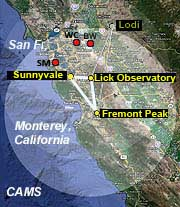
\includegraphics[scale=0.7]{images/CAMS_trio.jpg}
%   \setcaptioncitation{http://cams.seti.org/maps.html}
  \caption{The three CAMS network stations within a $50$ mile radius.}
  \label{trio}
\end{figure}

Accurate trajectories are particularly useful in back-tracing the motion of the meteor's orbit.  
The CAMS team has reduced over $320,000$ of these orbits \cite{noauthor_cameras_nodate}. 
In addition to calculating orbits, CAMS also uses their precise velocity measurements to draw relations between speed and other properties. 
Figure \ref{fancyCAMS} shows the relationship between the apparent incident speed and peak magnitude.

\begin{figure}[ht!]
  \centering
  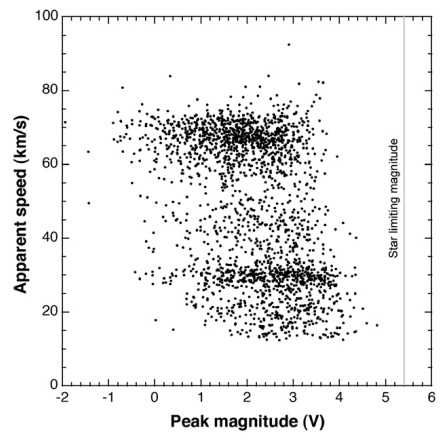
\includegraphics[scale=0.6]{images/CAMS_plot.png}
  \caption{Relationship between incident apparent speed and peak magnitude for CAMS data taken in November of 2010 \cite{jenniskens_cams:_2011}.}
  \label{fancyCAMS}
\end{figure}


Although the plot itself doesn't show a linear relationship, when considering the two subsets of relatively higher and lower incident speeds, we can see a general trend.
That trend shows that lower incident speed meteors tend to have slightly dimmer peak magnitudes. 



\subsection{SPMN}

The SPanish Meteor Network (SPMN) works extremely similarly to the CAMS project.  
It consists of $25$ observation stations located across Portugal and Spain \cite{trigo-rodriguez_2006_2007}.
Figure \ref{SPan} shows the approximate coverage of these stations along with some proposed locations (in green), from a satellite point of view.  

\begin{figure}[ht!]
  \centering
  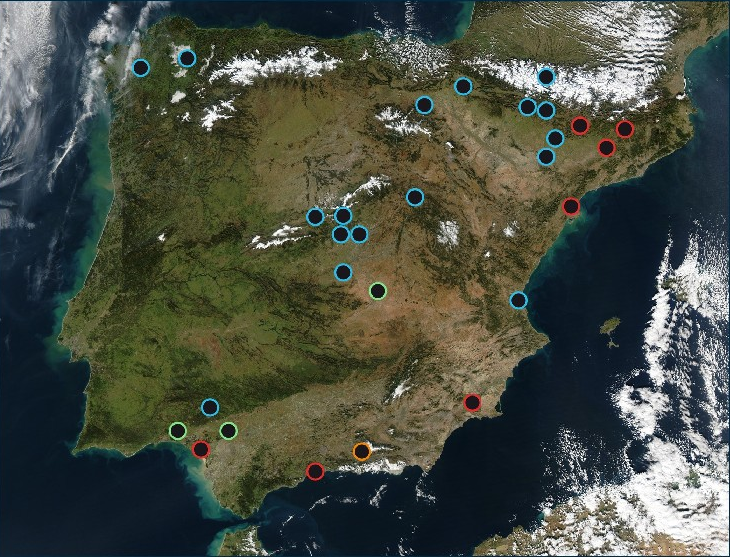
\includegraphics[scale=0.3]{images/satalite_of_love.png}
  \caption{Satellite view of the SPanish Meteor Network's sky coverage across $25$ existing and $3$ proposed observation stations  \cite{noauthor_presentation_nodate}.}
  \label{SPan}
\end{figure}

In addition to becoming the first organization in Spain to successfully calculate the orbital path of a meteor, this organization revolutionized fireball research by developing the first CCD AllSky cameras \cite{noauthor_presentation_nodate}.
These cameras are now in use all across the world.
While the SPMN and CAMS are extremely powerful research organizations, their study of meteors only slightly overlaps with the research being discussed in this paper.
Because of their high grade equipment, they are able to capture data from extremely dim sources.
Fireballs, quantified by a magnitude below $-4$, compose only a small fraction of the meteors analyzed by these organizations.
Fortunately, other organizations focus specifically on larger and brighter events.

\subsection{Other research groups}

There are a multitude of ways that one can attain information about a fireball.  
All the aforementioned surveys have employed the use of photometric data.
Peter Brown, a well renowned fireball researcher, took data from the Department of Defense and the Department of Energy space-based systems in geostationary orbits.
The original purpose of these systems is to detect signatures of explosions near earth's surface, but occasionally pick up false positives in the form of bolides.  
Because the systems detect the amount of power released, scientists such as Peter Brown can approximate the fireball's energy.
In a 2002 article published by \textit{Nature}, Brown estimated the optical energies of around 300 bolides.
From this data set and other existing data sets, Brown created Eq. \ref{browneq}, which relates bolide energy to the number of impacts on earth each year. 

\begin{figure}[ht!]
  \centering
  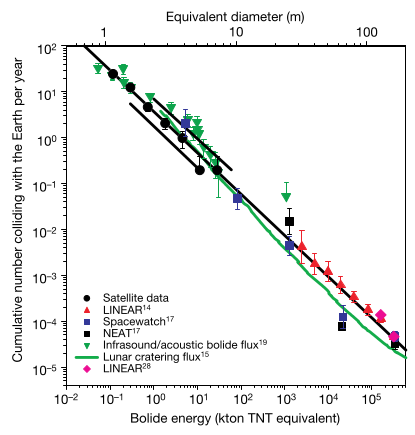
\includegraphics[scale=0.7]{images/flux_brown.png}
  \caption{A plot of bolide flux using an conglomeration of data \cite{brown_p_flux_2002}.}
  \label{powerlaw}
\end{figure}


Figure \ref{powerlaw} shows this relationship alongside data taken from many different research groups.  
In his research, Brown used existing assumptions (mentioned in the Analysis section) for the blackbody distribution and the velocity.  



